
\section{\glsentrytext{AVIS} Measurement set-up}
The measurements of the \gls{AVIS} are carried out using a \Simulink model running at a sampling time of $\Ts = 1\unit{ms}$ as shown in \figref{fig:avis:simulink:setup} and \figref{fig:avis:simulink:avis}.

\begin{figure}
\setlength\figurewidth{\columnwidth}
  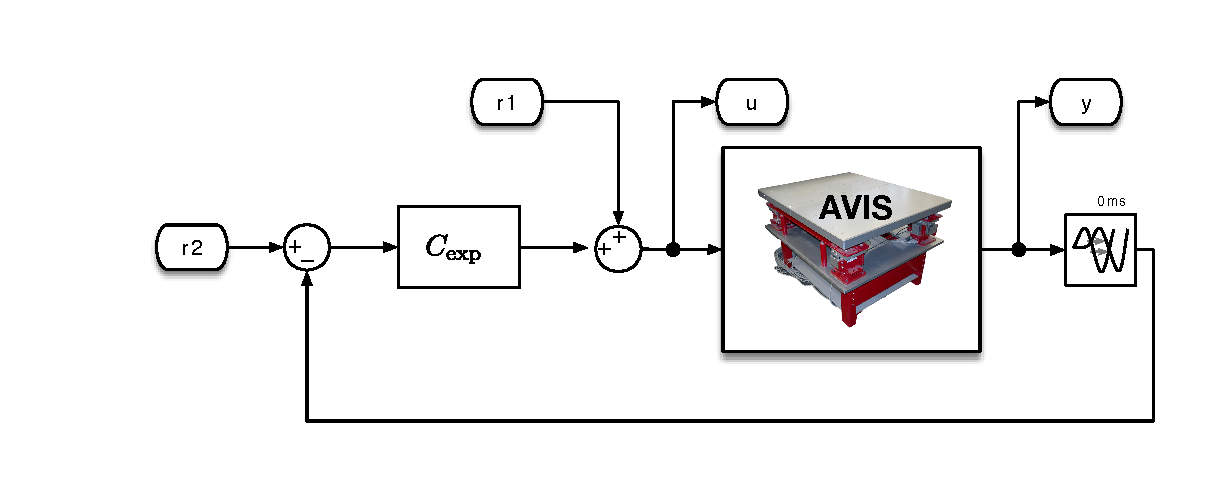
\includegraphics[width=\figurewidth]{\thisDir/figs/simulink-setup.pdf}
  \caption{Simulink model used during the AVIS measurements. All signals are six-dimensional real values.}
  \label{fig:avis:simulink:setup}
\end{figure}

In the top-level model (\figref{fig:avis:simulink:setup}), all signals are six-dimensional and each element corresponds to a mechanical degree-of-freedom of the \gls{AVIS}, i.e.
\begin{enumerate}
  \item the translational velocity in $x$ direction (horizontal),
  \item the translational velocity in $y$ direction (horizontal),
  \item the translational velocity in $z$ direction (vertical),
  \item the rotational velocity around the $x$ axis,
  \item the rotational velocity around the $y$ axis,
  \item the rotational velocity around the $z$ axis.
\end{enumerate}
In the main text, we have simplified this system to consider only the translation in the vertical direction (i.e. the third signal).
For the other directions, the applied signals (\code{r1} and \code{r2}) were set to $0$.
However, inside the feedback loop, all directions are controlled by the experimental controller $\experimental\Controller$.

Specifically, $\experimental\Controller$ is a $6\times6$ transfer function that is implemented as a discrete state-space model.
This controller was present beforehand~\citep{Rademakers2005MSc,vanderMaas2011MSc} and is given by the state-space matrices below
\begin{align}
  \experimental\Controller & \isdef \stateSpace{A}{B}{C}{D}\\
  A       &\approx 828.8 \cdot 10^{-3} \cdot \Identity{6} \\
  B = C &\approx \AvisMatrixDiagonal{93.83}{39.57} \cdot 10^{-3}\\
  D       &= \AvisMatrixDiagonal{4.982}{0.886} \cdot 10^{-3}
\end{align}
with $\Identity{n}$ the $n\times n$ identify matrix.
It can be seen that the controller is diagonal, i.e. the directions are decoupled, and that the dynamics are common among the translational directions and the rotational directions respectively, such that
\begin{equation}
  \experimental\Controller = 
  \AvisMatrixDiagonal{\experimental\Controller_{\mathrm{tran}}}{\experimental\Controller_{\mathrm{rot}}}
\end{equation}
with
\begin{align}
\experimental\Controller_{\mathrm{tran}} &  \approx 
   \frac{4.9821 z + 4.6787}{ z - 0.8282} \cdot 10^{-3} \\
  \experimental\Controller_{\mathrm{rot}} & \approx 
    \frac{0.88595 z + 0.83201}{ z - 0.8282} \cdot 10^{-3}
\end{align}
 as visualized in \figref{fig:avis:bodeplots:controllerAndSensor}.

\begin{figure}
\setlength\figurewidth{0.75\columnwidth}
\setlength\figureheight{0.68\figurewidth}
% This file was created by matlab2tikz.
%
%The latest updates can be retrieved from
%  http://www.mathworks.com/matlabcentral/fileexchange/22022-matlab2tikz-matlab2tikz
%where you can also make suggestions and rate matlab2tikz.
%
\begin{tikzpicture}


\pgfplotsset{amplitudePlot/.append style={%
  height=0.5\figureheight,
  ylabel={Amplitude \axisunit{dB}}}}
\pgfplotsset{phasePlot/.append style={%
  height=0.5\figureheight,
  ylabel={Phase \axisunit{rad}},
  ytick={-3.1416,-1.5708,0,1.5708,3.1416},
  yticklabels={{$-\pi$},$-\pi/2$,$0$,$\pi/2$,$\pi$},
  ymin=-3.142,
  ymax=3.142
  }}
\pgfplotsset{controllerAmpl/.append style={ymin=-80,ymax=-20}}
\pgfplotsset{filterAmpl/.append style={ymin=-20,ymax=20, yticklabel pos=right, ylabel near ticks, ytick={-20,0,20}}}
\pgfplotsset{noXTicks/.append style={xticklabels={}}}
\pgfplotsset{noYTicks/.append style={yticklabels={}}}
\pgfplotsset{noXLabel/.append style={xlabel={}, noXTicks}}
\pgfplotsset{noYLabel/.append style={ylabel={}, noYTicks}}


\begin{groupplot}[%
group style={%
  group name=derivs,
  group size=3 by 2,
  horizontal sep=0.5em,
  vertical sep=1em},
xlabel={Frequency $\omega \axisunit{Hz}$},
scale only axis,
xmode=log,
xmin=0.00016,
xmax=500,
xtick={0.01, 1, 100},
xminorticks=true,
grid=major,
width=0.33\figurewidth]


% ================================================
\nextgroupplot[amplitudePlot, controllerAmpl, noXLabel, title={$\experimental\Controller_{\mathrm{tran}}$}]
\addplot[myDerivs] table[] {\thisDir/data/avis-setup/Ctran-mag.tsv};

% ================================================
\nextgroupplot[amplitudePlot, controllerAmpl, noYLabel, noXLabel, title={$\experimental\Controller_{\mathrm{rot}}$}]
\addplot[myDerivs] table[] {\thisDir/data/avis-setup/Crot-mag.tsv};

% ================================================
\nextgroupplot[amplitudePlot, filterAmpl, noXLabel, title={$F_{\phantom{rot}}$}]
\addplot[myDerivs] table[] {\thisDir/data/avis-setup/sensFilter-mag.tsv};

% ================================================
% ================================================

% ================================================
\nextgroupplot[phasePlot]
\addplot[myDerivs] table[] {\thisDir/data/avis-setup/Ctran-phase.tsv};

% ================================================
\nextgroupplot[phasePlot, noYLabel, noYTicks]
\addplot[myDerivs] table[] {\thisDir/data/avis-setup/Crot-phase.tsv};

% ================================================
\nextgroupplot[phasePlot, noYLabel, noYTicks]
\addplot[myDerivs] table[] {\thisDir/data/avis-setup/sensFilter-phase.tsv};

\end{groupplot}

\end{tikzpicture}%

\caption{Bode plots of the elements of $\experimental\Controller$ and sensor filter $F$ present in the set-up.}
\label{fig:avis:bodeplots:controllerAndSensor}
\end{figure}

For multisine excitations the \code{RepeatingSequence} block was used to load the \code{r2} signal from \MATLAB, for noise excitations, the \code{RandomNumber} block of \Simulink was used instead.
The signals \code{r2}, \code{u} and \code{y} are returned from \Simulink to \MATLAB where further processing of the data is carried out.
This allows to compute the transfer function from \code{r2} to \code{u} and \code{y} respectively, or, the transfer function of the \gls{AVIS} block in the \Simulink model.

The \gls{AVIS} block (\figref{fig:avis:simulink:avis}), conceptually, contains:
\begin{itemize}
  \item static transformations $(K_{\mathrm{act}}, K_{\mathrm{sens}})$, as derived from first principles in \citep{Rademakers2005MSc}, which translates the sensor and actuator signals to physical velocities at the center of the payload,
  \item logic to communicate with the Quanser Q8 \gls{DAQ} board which is physically connected to the \gls{AVIS}, and
  \item signal conditioning.
\end{itemize}

Specifically, the static transformations of the \gls{AVIS} are given by the following gain matrices~\citep[Appendix A.4]{Rademakers2005MSc}:
\begin{align}
  K_{\mathrm{act}}    & \approx \begin{bmatrix}
     \deemph{0} &   -0.5 &      \deemph{0} &      \deemph{0} &      \deemph{0} & -0.6485\\
0.0974 & 0.1233 &  -0.25 & -0.6667 & 0.5263 &      \deemph{0}\\
  -0.5 &      \deemph{0} &      \deemph{0} &      \deemph{0} &      \deemph{0} & -0.5119\\
0.0974 & -0.1233 & -0.255 & 0.6667 & 0.5263 &      \deemph{0}\\
     \deemph{0} &    0.5 &      \deemph{0} &      \deemph{0} &      \deemph{0} & -0.6485\\
-0.0974 & -0.1233 &  -0.25 & 0.6667 & -0.5263 &      \deemph{0}\\
   0.5 &      \deemph{0} &      \deemph{0} &      \deemph{0} &      \deemph{0} & -0.5119\\
-0.0974 & 0.1233 &  -0.25 & -0.6667 & -0.5263 &      \deemph{0}\\
\end{bmatrix}
\\
  K_{\mathrm{sens}} & \approx \begin{bmatrix}
   0.3947 &      \deemph{0} &     -1 & -0.1158 & 0.3947 & 0.1158\\
  -0.5 & -0.1467 &      \deemph{0} & 0.1467 &    0.5 &      \deemph{0}\\
     \deemph{0} &    0.5 &      \deemph{0} &      \deemph{0} &      \deemph{0} &    0.5\\
     \deemph{0} & 1.3333 &      \deemph{0} & -1.3333 &      \deemph{0} &      \deemph{0}\\
     \deemph{0} &      \deemph{0} &      \deemph{0} & -1.0526 &      \deemph{0} & 1.0526\\
-1.0526 &      \deemph{0} &      \deemph{0} &      \deemph{0} & -1.0526 &      \deemph{0}\\
\end{bmatrix}

\end{align}
Note that $K_{\mathrm{act}} \in \RR^{8\times6}$ and hence produces signals for the $8$ actuators on the \gls{AVIS}.
These signals are limited to the range $\pm 5\unit{V}$ before they are sent to the \glspl{DAC} on the Q8 \gls{DAQ} board to avoid overdriving the \glspl{DAC}.

The $6$ velocity signals that are digitized by the Q8 \gls{DAQ} are each filtered to transform the voltage induced in the coils of the geophones on the \gls{AVIS} into a velocity using a filter $F$ with transfer function
\begin{equation}
  F(s) \approx \frac{6.51 s^2 + 122 s + 11.3}{6.4 s^2 - 16.6 s - 2.2}

\end{equation}
which is shown in \figref{fig:avis:bodeplots:controllerAndSensor}.
More information regarding this design is given in \citep[Appendix A.3]{Rademakers2005MSc}.
This filter is discretized automatically by \Simulink for the actual implementation.

The output \code{y} is clipped to $\pm 20$ for easier detection of errors.
However, during normal operation and all the measurements, the signal levels were well within the linear region of this saturation block.

\begin{figure}
\setlength\figurewidth{\columnwidth}
  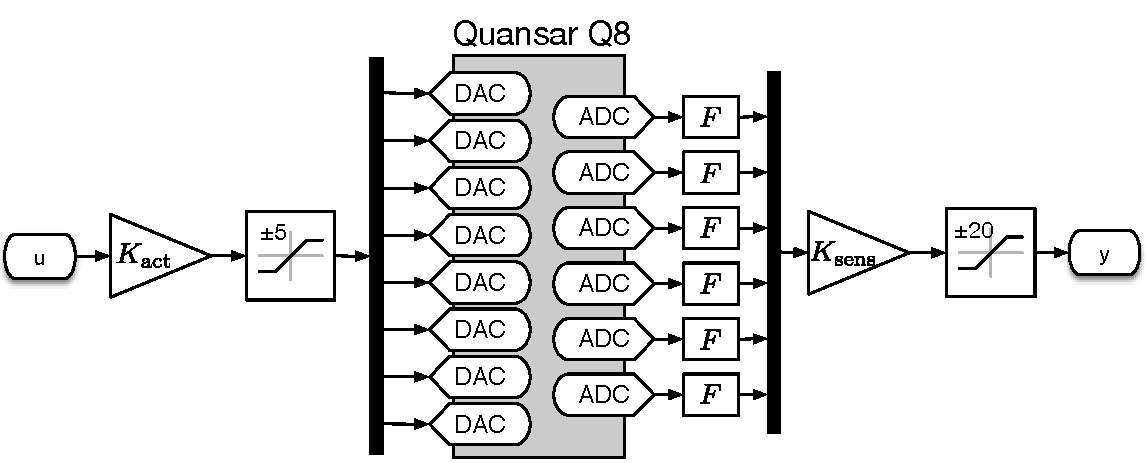
\includegraphics[width=\figurewidth]{\thisDir/figs/simulink-avis.pdf}
  \caption{Simulink model of the AVIS sub-block.}
  \label{fig:avis:simulink:avis}
\end{figure}

